\documentclass{ctexart}
\usepackage{graphicx}
\usepackage{caption}
\usepackage{float}
\usepackage{amsmath}
\usepackage{fancyhdr}
\usepackage{xunicode-addon}
\usepackage{booktabs}
\usepackage[a4paper,hmargin=1.25in,vmargin=1in]{geometry}
% !TeX program = xelatex
\title{\begin{figure}[H]
	\centering 
	\includegraphics[height=7cm,width=14cm]{E:/Pictures/中科大.jpg}
	\end{figure}\Huge\textbf{Lab 7}\\\huge{}}
\date{}
\punctstyle{banjiao} 
\pagestyle{fancy}
	\fancyhead[C]{\LARGE\textbf{Lab 7}}
	\fancyhead[L]{}
	\fancyhead[R]{}
	\fancyfoot[C]{\thepage}
\begin{document}
	\maketitle
	\thispagestyle{empty}
	
	\[\makebox{\Large{姓名:\underline{\makebox[5cm]{高茂航}}}}\]
	
    \[\makebox{\Large{学号:\underline{\makebox[5cm]{PB22061161}}}}\]
	
	$$\makebox{\Large{日期:\underline{\makebox[5cm]{2024.6.10}}}}$$
	
	\clearpage

	\pagenumbering{arabic}
	\section{Problem Descriptions}
已知加速度,用Romberg数值积分计算速度和位移。
	\section{Analysis and Algorithms}
	现在要用数值方法求$\int_{a}^{b} f(x) \, dx$,
	
	设$h=\frac{b-a}{n}$,已知:
	
复化梯形积分$T_{n}\left(f\right)=h\left[\frac{1}{2}f\left(a\right)+\sum_{i=1}^{n-1}f\left(a+ih\right)+\frac{1}{2}f\left(b\right)\right]$、

	复化Simpson积分$S_{n}\left(f\right)=\frac{h}{3}\left[f\left(a\right)+4\sum_{i=0}^{m-1}f\left(x_{2i+1}\right)+2\sum_{i=1}^{m-1}f\left(x_{2i}\right)+f\left(b\right)\right]$.

	将 $( T_n( f) - T_{2n}( f) )$ 作 为 $T_{2n}(f)$的修正值补充到$I(f)$,即
$$I(f)\approx T_{2n}(f)+\frac{1}{3}\left(T_{2n}\left(f\right)-T_{n}\left(f\right)\right)=\frac{4}{3}T_{2n}-\frac{1}{3}T_{n}=S_{n}$$


其结果是将复化梯形求积公式组合成复化 Simpson 求积公式, 截断误差由$O(h^2)$提高到$O(h^4)$.这种手段称为外推算法,该算法在不增加计算量的前提下提高了误差的精度.
不妨对$S_{2n}(f),S_n(f)$再作一次线性组合:

$$I\left(f\right)-S_{n}\left(f\right)=-\frac{f^{\left(4\right)}\left(\xi\right)}{180}h^{4}\left(b-a\right)\approx dh^{4}$$
$$I(f)-S_{2n}(f)=-\frac{f^{(4)}(\eta)}{180}\left(\frac{h}{2}\right)^{4}(b-a)\approx d\left(\frac{h}{2}\right)^{4}$$


$$I\left(f\right)\approx S_{2n}\left(f\right)+\frac{1}{15}\left(S_{2n}\left(f\right)-S_{n}\left(f\right)\right)=C_{n}\left(f\right)$$
复化 Simpson 公式组成复化 Cotes 公式,其截断误差是$O(h^6).$同理对 Cotes
公式进行线性组合:
$$I\left(f\right)-C_{2n}\left(f\right)=e\left(\frac{h}{2}\right)^{6}\\I\left(f\right)-C_{n}\left(f\right)=eh^{6}$$
得到具有 7 次代数精度和截断误差是$O(h^8)$的 Romberg 公式:
$$R_{n}\left(f\right)=C_{2n}\left(f\right)+\frac{1}{63}\left(C_{2n}\left(f\right)-C_{n}\left(f\right)\right)$$

为了便于在计算机上实现 Romberg 算法,将$T_n,S_n,C_n,R_n,\cdots$统一用$R_{k,j}$ 表示,
列标$j=1,2,3,4$分别表示梯形、Simpson、Cotes 、Romberg积分,行标$k$表示步长$h_k=\frac h{2^{k-1}}$,得到Romberg 计算公式:
$$R_{k,j}=R_{k,j-1}+\frac{R_{k,j-1}-R_{k-1,j-1}}{4^{j-1}-1},k=2,3,\cdots $$
对每一个$k,j$从 2 做到$k$,一直做到$|R_k,k-R_{k-1,k-1}|$小于给定控制精度时停止
计算.
	\section{Results}
	\begin{figure}[H]
		\centering 
		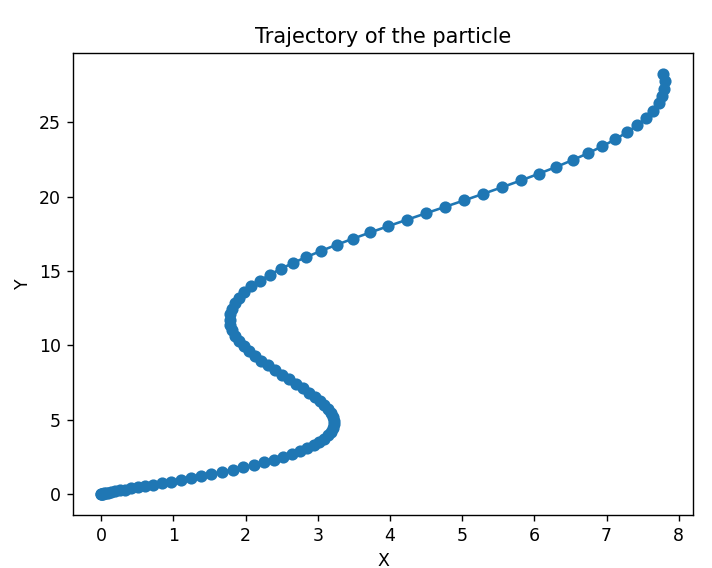
\includegraphics[height=7cm,width=14cm]{1.png}
		\caption{M=8时的粒子轨迹}
		\end{figure}
		\begin{figure}[H]
			\centering 
			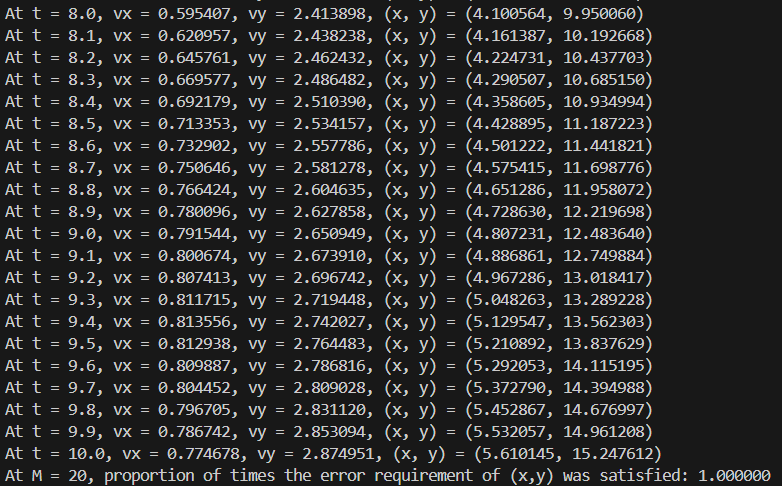
\includegraphics[height=7cm,width=10cm]{2.png}
			\caption{部分输出结果}
			\end{figure}
			
		\section{Conclusion}
		M=4时Romberg积分达到要求精度的比例为0.05,M=8时为0.88,M=12,16,20时均为1,从结果可看出M越大,Romberg积分达到要求精度的比例越高。
		但由于M越大,计算量越大,耗时越长,因此需要根据实际情况,平衡达到要求精度的比例和M的大小,例如在本实验中可以取M=12。

    \end{document}